\emph{In problems 1-3, use the nearest neighbor algorithm to find a minimum possible circuit through each graph starting at $a$.}

\begin{center}
\begin{tabular}{c c c}
\parbox{1.5in}{\begin{enumerate}
\item \text{} \begin{center}
\begin{tikzpicture}
  \GraphInit[vstyle=simple]
  \tikzset{VertexStyle/.append style={scale=0.3}}
  \grEmptyCycle[prefix=a,RA=1.5]{4}
  
  \extralabel{a0}{0}{$a$}
  \extralabel{a1}{90}{$b$}
  \extralabel{a2}{180}{$c$}
  \extralabel{a3}{-90}{$d$}
  
  \Edge[label=3](a0)(a1)
  \Edge[label=6](a1)(a2)
  \Edge[label=7](a2)(a3)
  \Edge[label=2](a3)(a0)
  \tikzstyle{LabelStyle}=[fill=white,pos=0.3]
  \Edge[label=4](a1)(a3)
  \Edge[label=5](a0)(a2)
\end{tikzpicture}
\end{center}
\end{enumerate}}
&
\parbox{1.5in}{\begin{enumerate}
\setcounter{enumi}{1}
\item \text{} \begin{center}
\begin{tikzpicture}
  \GraphInit[vstyle=simple]
  \tikzset{VertexStyle/.append style={scale=0.3}}
  \grEmptyCycle[prefix=a,RA=1.5,rotation=18]{5}
  
  \extralabel{a0}{0}{$a$}
  \extralabel{a1}{90}{$b$}
  \extralabel{a2}{180}{$c$}
  \extralabel{a3}{-90}{$d$}
  \extralabel{a4}{-90}{$e$}
  
  \Edge[label=3](a0)(a1)
  \Edge[label=10](a1)(a2)
  \Edge[label=6](a2)(a3)
  \Edge[label=1](a3)(a4)
  \Edge[label=7](a4)(a0)
  \Edge[label=8](a0)(a2)
  \Edge[label=4](a0)(a3)
  \Edge[label=9](a1)(a3)
  \Edge[label=2](a1)(a4)
  \Edge[label=5](a2)(a4)
\end{tikzpicture}
\end{center}
\end{enumerate}}
&
\parbox{1.5in}{\begin{enumerate}
\setcounter{enumi}{2}
\item \text{} \begin{center}
\begin{tikzpicture}
  \GraphInit[vstyle=simple]
  \tikzset{VertexStyle/.append style={scale=0.3}}
  \grEmptyCycle[prefix=a,RA=1.5]{6}
  
  \extralabel{a0}{0}{$a$}
  \extralabel{a1}{90}{$b$}
  \extralabel{a2}{90}{$c$}
  \extralabel{a3}{180}{$d$}
  \extralabel{a4}{-90}{$e$}
  \extralabel{a5}{-90}{$f$}
  
  \Edge[label=3](a0)(a1)
  \Edge[label=4](a0)(a5)
  \Edge[label=5](a1)(a2)
  \Edge[label=1](a2)(a3)
  \Edge[label=4](a3)(a4)
  \Edge[label=7](a4)(a5)
  \tikzstyle{LabelStyle}=[fill=white,pos=0.3]
  \Edge[label=2](a0)(a2)
  \Edge[label=3](a0)(a4)
  \Edge[label=6](a3)(a1)
  \Edge[label=3](a3)(a5)
  \tikzstyle{LabelStyle}=[fill=white,pos=0.35]
  \Edge[label=5](a0)(a3)
  \Edge[label=8](a2)(a5)
  \Edge[label=4](a4)(a1)
\end{tikzpicture}
\end{center}
\end{enumerate}}\\
\boxtext{$a \to d \to b \to c$} & \boxtext{$a \to b \to e \to d \to c$} & \boxtext{$a \to c \to d \to f \to e \to b$}
\end{tabular}
\end{center}
\pagebreak

\emph{In problems 4--6, use Dijkstra's algorithm to find the shortest path through each graph between $a$ and $z$.}

\begin{center}
\begin{tabular}{c c c}
\parbox{1.5in}{\begin{enumerate}
\setcounter{enumi}{3}
\item \text{} \begin{center}
\begin{tikzpicture}
  \GraphInit[vstyle=simple]
  \tikzset{VertexStyle/.append style={scale=0.3}}
  \SetGraphUnit{0.8}
  
  \Vertex{a}
  \NOEA(a){b}
  \SOEA(a){c}
  \EA(b){d}
  \EA(c){e}
  \NOEA(e){z}
  
  \extralabel{a}{180}{$a$}
  \extralabel{b}{90}{$b$}
  \extralabel{c}{-90}{$c$}
  \extralabel{d}{90}{$d$}
  \extralabel{e}{-90}{$e$}
  \extralabel{z}{0}{$z$}
  
  \Edge[label=2](a)(b)
  \Edge[label=3](a)(c)
  \Edge[label=5](b)(d)
  \Edge[label=2](b)(e)
  \Edge[label=5](c)(e)
  \Edge[label=1](d)(e)
  \Edge[label=2](d)(z)
  \Edge[label=4](e)(z)
\end{tikzpicture}
\end{center}
\end{enumerate}}
&
\parbox{1.5in}{\begin{enumerate}
\setcounter{enumi}{4}
\item \text{} \begin{center}
\begin{tikzpicture}
  \GraphInit[vstyle=simple]
  \tikzset{VertexStyle/.append style={scale=0.3}}
  \SetGraphUnit{0.8}
  
  \Vertex{a}
  \NOEA(a){b}
  \SOEA(a){c}
  \EA(b){d}
  \EA(c){e}
  \EA(d){f}
  \EA(e){g}
  \NOEA(g){z}
  
  \extralabel{a}{180}{$a$}
  \extralabel{b}{90}{$b$}
  \extralabel{c}{-90}{$c$}
  \extralabel{d}{90}{$d$}
  \extralabel{e}{-90}{$e$}
  \extralabel{f}{90}{$f$}
  \extralabel{g}{-90}{$g$}
  \extralabel{z}{0}{$z$}
  
  \Edge[label=4](a)(b)
  \Edge[label=3](a)(c)
  \Edge[label=5](b)(d)
  \Edge[label=2](b)(c)
  \Edge[label=3](c)(d)
  \Edge[label=6](c)(e)
  \Edge[label=1](d)(e)
  \Edge[label=5](d)(f)
  \Edge[label=5](e)(g)
  \Edge[label=2](f)(g)
  \Edge[label=7](f)(z)
  \Edge[label=4](g)(z)
\end{tikzpicture}
\end{center}
\end{enumerate}}
&
\parbox{1.5in}{\begin{enumerate}
\setcounter{enumi}{5}
\item \text{} \begin{center}
\begin{tikzpicture}
  \GraphInit[vstyle=simple]
  \tikzset{VertexStyle/.append style={scale=0.3}}
  \grEmptyCycle[prefix=a,RA=1.1,rotation=18]{5}
  
  \extralabel{a0}{45}{$a$}
  \extralabel{a1}{90}{$b$}
  \extralabel{a2}{135}{$c$}
  \extralabel{a3}{-90}{$z$}
  \extralabel{a4}{-90}{$e$}
  
  \Edge[label=7](a0)(a1)
  \Edge[label=3](a1)(a2)
  \Edge[label=5](a2)(a3)
  \Edge[label=4](a2)(a4)
  \Edge[label=9](a3)(a4)
  \Edge[label=3](a4)(a0)
  \tikzstyle{LabelStyle}=[fill=white,pos=0.6]
  \Edge[label=6](a0)(a2)
  \Edge[label=7](a1)(a4)
\end{tikzpicture}
\end{center}
\end{enumerate}}\\
\boxtext{$a \to b \to e \to d \to z$} & \boxtext{$a \to c \to d \to e \to g \to z$} & \boxtext{$a \to c \to z$}
\end{tabular}
\end{center}

\begin{enumerate}
\setcounter{enumi}{6}

\item The graph below shows the distances between cities.  Use the graph to answer the questions below.
\begin{center} %7
\begin{tikzpicture}[scale=0.95]
  \GraphInit[vstyle=simple]
  \tikzset{VertexStyle/.append style={scale=0.3}}
  \Vertex[x=0,y=0]{Denver}
  \Vertex[x=1.8,y=2]{Minneapolis}
  \Vertex[x=3,y=-0.75]{STL}
  \Vertex[x=3.75,y=1]{Chicago}
  \Vertex[x=4.5,y=0]{Indianapolis}
  \Vertex[x=4.2,y=-2]{Nashville}
  \Vertex[x=1.5,y=-3.5]{Dallas}
  \Vertex[x=5,y=-3]{Atlanta}
  \Vertex[x=5.2,y=1.2]{Detroit}
  \Vertex[x=6.5,y=0.5]{NYC}
    
  \extralabel[0mm]{Denver}{135}{Denver}
  \extralabel[2mm]{Minneapolis}{90}{Minneapolis}
  \extralabel[2mm]{STL}{-90}{St. Louis}
  \extralabel[3mm]{Chicago}{90}{Chicago}
  \extralabel[0mm]{Indianapolis}{-30}{Indianapolis}
  \extralabel[2mm]{Nashville}{30}{Nashville}
  \extralabel[2mm]{Dallas}{180}{Dallas}
  \extralabel[2mm]{Atlanta}{-30}{Atlanta}
  \extralabel[2mm]{Detroit}{45}{Detroit}
  \extralabel[0mm]{NYC}{45}{\parbox{0.5in}{New\\ York}}
  
  \Edge[label=795](Denver)(STL)
  \Edge[label=690](Denver)(Minneapolis)
  \Edge[label=665](Denver)(Dallas)
  \Edge[label=360](Minneapolis)(Chicago)
  \Edge[label=480](Minneapolis)(STL)
  \Edge[label=245](Chicago)(Detroit)
  \Edge[label=165](Chicago)(Indianapolis)
  \Edge[label=250](Chicago)(STL)
  \Edge[label=255](Indianapolis)(STL)
  \Edge[label=260](Indianapolis)(Nashville)
  \Edge[label=215](Nashville)(Atlanta)
  \Edge[label=640](Indianapolis)(NYC)
  \Edge[label=480](Detroit)(NYC)
  \Edge[label=620](Dallas)(Nashville)
  \Edge[label=715](Dallas)(Atlanta)
  \SetUpEdge[style={bend right=50}]
  \Edge[label=730](Atlanta)(NYC)
\end{tikzpicture}
\end{center}
\begin{enumerate}[(a)]
\item Use the nearest neighbor algorithm to find a path that starts in Chicago and visits all the cities shown, while trying to minimize distance traveled. \answersub{CHI $\to$ IND $\to$ STL $\to$ MIN $\to$ DEN $\to$ DAL $\to$ NAS $\to$ ATL $\to$ NYC $\to$ DET}
\item What is the total length of the path found in part (a)? \answersub{4300 miles}
\item Find the shortest path between Dallas and New York.  What is the length of this path? \answersub{DAL $\to$ ATL $\to$ NYC (1445 miles)}
\item Find the shortest path between Minneapolis and Atlanta.  What is the length of this path? \answersub{MIN $\to$ CHI $\to$ IND $\to$ NAS $\to$ ATL (1000 miles)}
\end{enumerate}
\pagebreak

\item The graph below shows the cost of flights between cities.  Use the graph to answer the questions below.
\begin{center} %8
\begin{tikzpicture}[scale=0.95]
  \GraphInit[vstyle=simple]
  \tikzset{VertexStyle/.append style={scale=0.3}}
  \Vertex[x=0,y=0]{Denver}
  \Vertex[x=1.8,y=2]{Minneapolis}
  \Vertex[x=3,y=-0.75]{STL}
  \Vertex[x=3.75,y=1]{Chicago}
  \Vertex[x=4.5,y=0]{Indianapolis}
  \Vertex[x=4.2,y=-2]{Nashville}
  \Vertex[x=1.5,y=-3.5]{Dallas}
  \Vertex[x=5,y=-3]{Atlanta}
  \Vertex[x=5.2,y=1.2]{Detroit}
  \Vertex[x=6.5,y=0.5]{NYC}
    
  \extralabel[0mm]{Denver}{135}{Denver}
  \extralabel[2mm]{Minneapolis}{90}{Minneapolis}
  \extralabel[2mm]{STL}{-90}{St. Louis}
  \extralabel[3mm]{Chicago}{90}{Chicago}
  \extralabel[0mm]{Indianapolis}{-30}{Indianapolis}
  \extralabel[2mm]{Nashville}{30}{Nashville}
  \extralabel[2mm]{Dallas}{180}{Dallas}
  \extralabel[2mm]{Atlanta}{-30}{Atlanta}
  \extralabel[2mm]{Detroit}{45}{Detroit}
  \extralabel[0mm]{NYC}{45}{\parbox{0.5in}{New\\ York}}
  
  \Edge[label=\$137](Denver)(STL)
  \Edge[label=\$126](Denver)(Minneapolis)
  \Edge[label=\$123](Denver)(Dallas)
  \Edge[label=\$90](Minneapolis)(Chicago)
  \Edge[label=\$103](Minneapolis)(STL)
  \Edge[label=\$77](Chicago)(Detroit)
  \Edge[label=\$68](Chicago)(Indianapolis)
  \Edge[label=\$80](Chicago)(STL)
  \Edge[label=\$79](Indianapolis)(STL)
  \Edge[label=\$80](Indianapolis)(Nashville)
  \Edge[label=\$74](Nashville)(Atlanta)
  \Edge[label=\$120](Indianapolis)(NYC)
  \Edge[label=\$102](Detroit)(NYC)
  \Edge[label=\$118](Dallas)(Nashville)
  \Edge[label=\$129](Dallas)(Atlanta)
  \SetUpEdge[style={bend right=50}]
  \Edge[label=\$130](Atlanta)(NYC)
\end{tikzpicture}
\end{center}
\begin{enumerate}[(a)]
\item Use the nearest neighbor algorithm to find a path that starts in St. Louis and visits all the cities shown, while trying to minimize the cost of travel. \answersub{STL $\to$ IND $\to$ CHI $\to$ DET $\to$ NYC $\to$ ATL $\to$ NAS $\to$ DAL $\to$ DEN $\to$ MIN}
\item What is the total cost of the path found in part (a)? \answersub{\$897}
\item Find the cheapest path between Nashville and Denver.  What is the cost of this path? \answersub{NAS $\to$ DAL $\to$ DEN (\$241)}
\item Find the cheapest path between Detroit and Denver.  What is the cost of this path? \answersub{DET $\to$ CHI $\to$ MIN $\to$ DEN (\$293)}
\end{enumerate}

\item A salesperson has responsibility over four cities in Maryland and northern Virginia, and they compiled the distances between them; these distances are shown in the table below.    If the salesperson needs to visit all four cities, and is currently in Ellicott City, use the nearest neighbor algorithm to plan their route.  How far will they travel in total along this path?
{\footnotesize\begin{center}
\begin{tabular}{l | c c c c}
& Annapolis & Alexandria & Ellicott City & Reston\\
\hline
Annapolis & -- & 45 & 26 & 46\\
Alexandria & 45 & -- & 37 & 19\\
Ellicott City & 26 & 37 & -- & 35\\
Reston & 46 & 19 & 35 & --
\end{tabular}
\end{center}} \text{} \answer{EC $\to$ Ann. $\to$ Alex. $\to$ Res. (90 miles)}

\item An American tourist is traveling through Great Britain, and would like to visit five cities.  The tourist has estimated the cost of a train ticket between pairs of these cities, and the results are shown in the table below.  Plan a route that will take the tourist through all five cities with as little cost as possible, starting and ending in London.  Use the nearest neighbor algorithm; what is the cost of this journey?
{\footnotesize\begin{center}
\begin{tabular}{l | c c c c c}
& London & Edinburgh & York & Cardiff & Chester\\
\hline
London & -- & \$175 & \$110 & \$65 & \$115\\
Edinburgh & \$175 & -- & \$95 & \$195 & \$105\\
York & \$110 & \$95 & -- & \$145 & \$60\\
Cardiff & \$65 & \$195 & \$145 & -- & \$85\\
Chester & \$115 & \$105 & \$60 & \$85 & --
\end{tabular}
\end{center}} \text{} \answer{Lon. $\to$ Car. $\to$ Ches. $\to$ York $\to$ Edin. $\to$ Lon. (\$480)}
\end{enumerate}